\documentclass[12pt]{article}
\usepackage{cwilliams-standard}

\setclass{IPD}
\settitle{Project Management Document\\
        \large Quantum Error Correction with Transformer Models}
\setauthors{Tzu-Chen Chiu, Arjun Sivakumar, Mara Schimmel, Christopher Williams}
\setheaderauthors{Chiu, Sivakumar, Schimmel, Williams}

\begin{document}

\maketitlepage

\section{Collaboration Softwares:}
\begin{itemize}
        \item \textbf{Github:} Christopher manages and reviews pull requests, all will create branches and work on assigned tasks before they are reviewed and merge.
        \item \textbf{IDE:} VSCode and PyCharm
        \item \textbf{Docker:} Chris has created the image which contains the development environment and project requirements (along with version details). Team members will run containers with this image and develop inside it, committing and pushing as necessary.
        \item \textbf{Project Management Software:} Jira + Excel to manage project backlog, sprint tasks, time estimates, actual time taken, status updates, ticket assignments, etc.
\end{itemize}

\section{Person Hours Available}
Every team member is available for a minimum of 10 hours per week within the timeframe of the semester (i.e. not counting breaks).

\begin{important}{Link to Work}
        As some of the images are unable to easily depict the information, we will provide the link to our
        Google Sheet with all of our separate sheets and raw data \href{https://docs.google.com/spreadsheets/d/1keQPuotPkZdqrqZ_ybHGJQ7_mYCZARqL/edit?usp=sharing&ouid=113464029339812046851&rtpof=true&sd=true}{here}.
\end{important}\label{link}

\section{Product Backlog}

\begin{figure}[H]
        \centering
        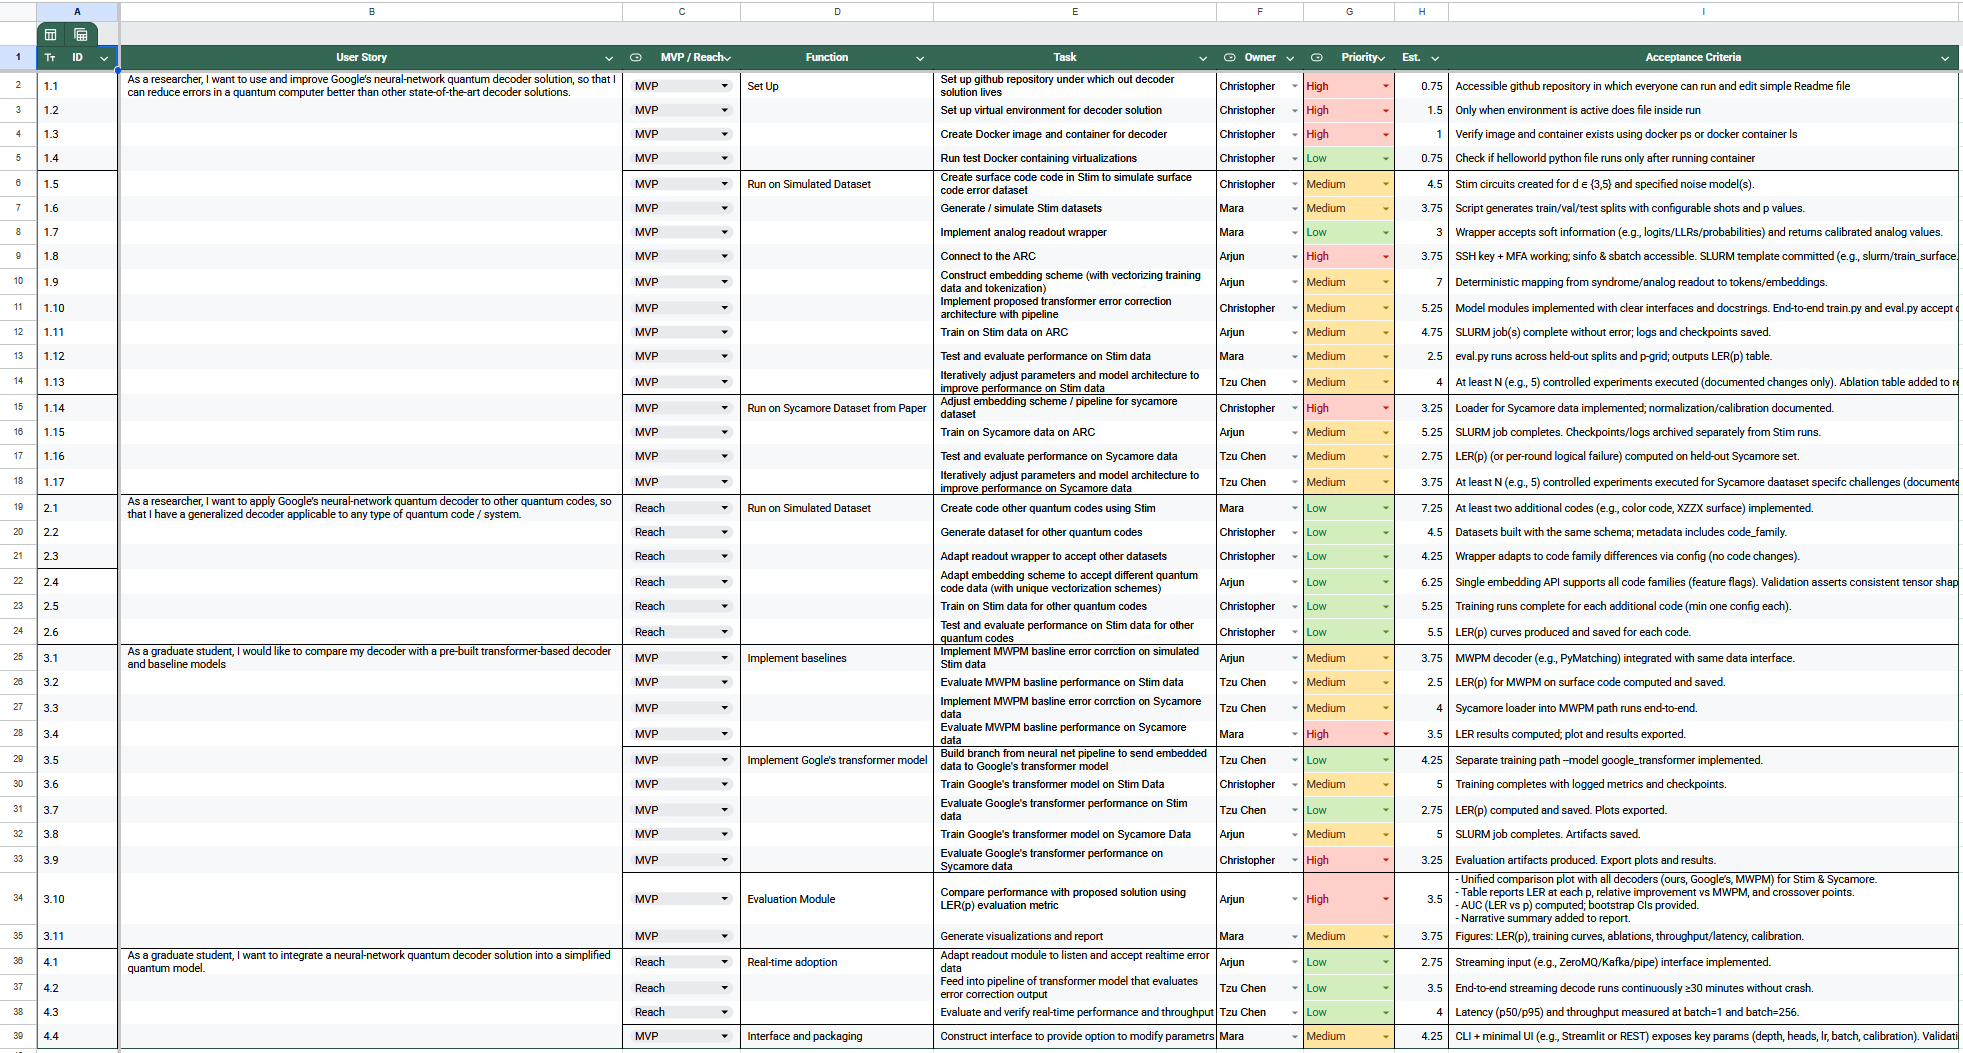
\includegraphics[width=1\linewidth]{images/Product_Backlog.png}
        \caption{Product Backlog including Tasks for all 3 sprints, as well as reach tasks.}
        \label{fig:1}
\end{figure}

We apologize for the readability of this table. The link from \hyperref[link]{earlier} will take you to our full table under the "Project Backlog" sheet.

\section{Story Point Estimates}

\begin{figure}[H]
        \centering
        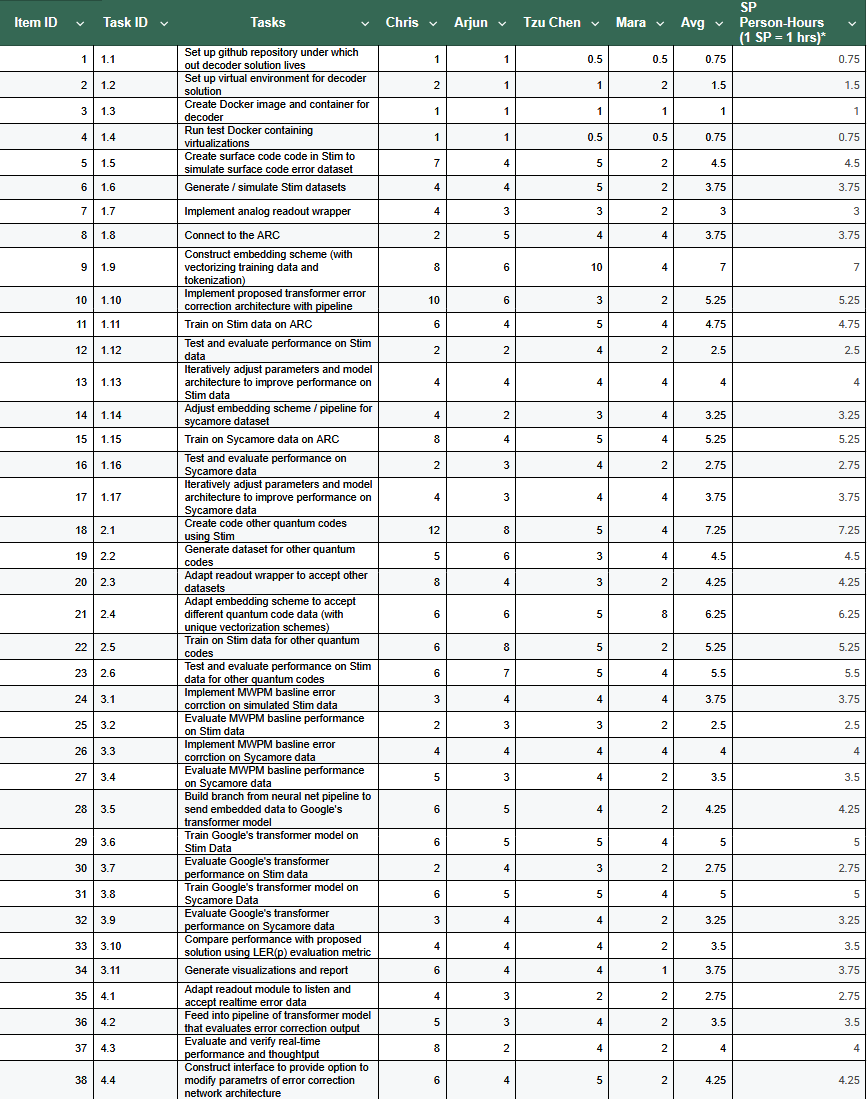
\includegraphics[width=0.9\linewidth]{images/story_point_estimates.png}
        \caption{Story Point Estimates for all Tasks}
        \label{fig:2}
\end{figure}

\section{Sprint Backlog}

\begin{figure}[H]
        \centering
        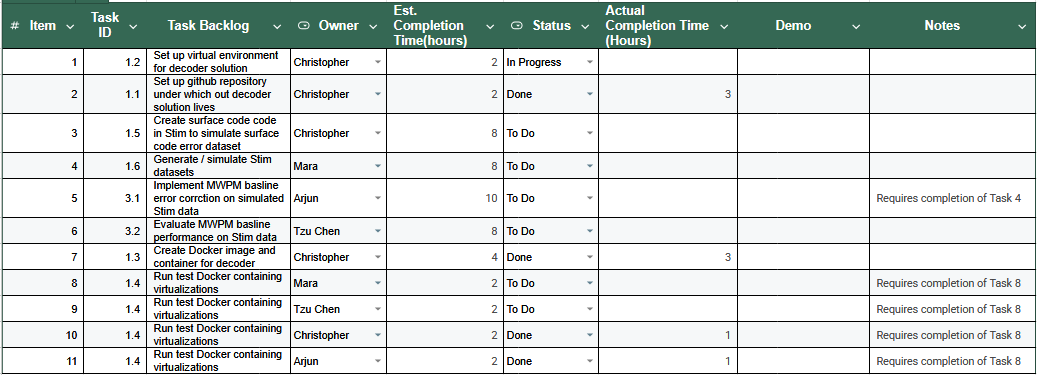
\includegraphics[width=1\linewidth]{images/sprint1_backlog.png}
        \caption{Sprint 1 Backlog}
        \label{fig:3}
\end{figure}

\section{Gantt Chart}

\begin{figure}[H]
        \centering
        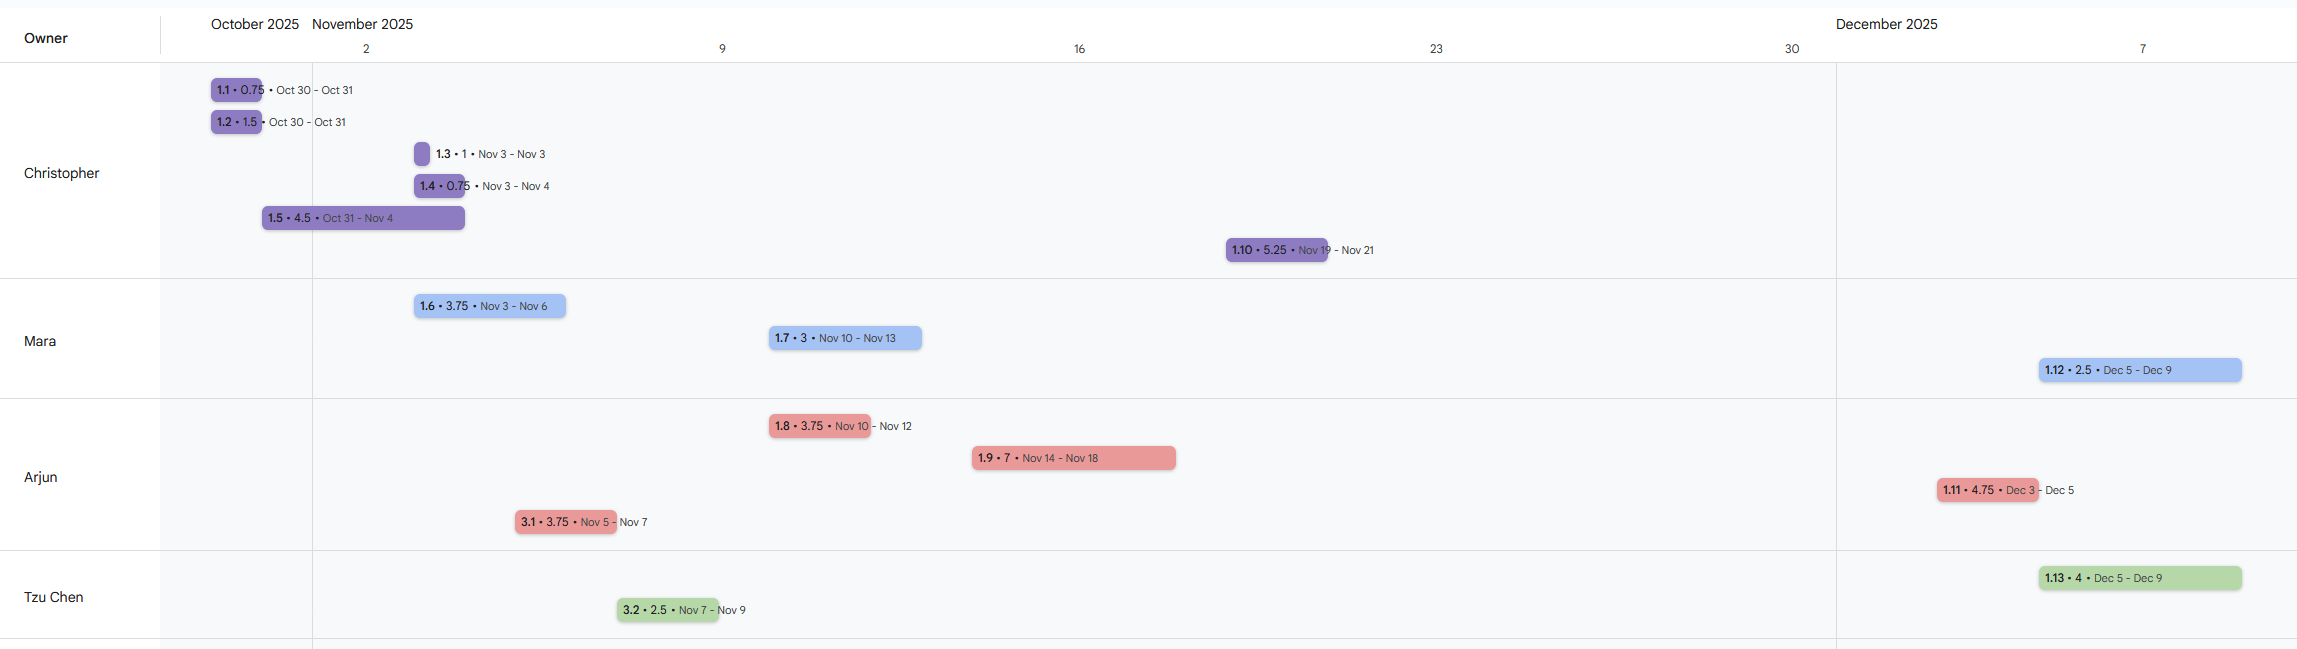
\includegraphics[width=1\linewidth]{images/gantt_chart_for_project.png}
        \caption{Gantt Chart for 3 Sprints}
        \label{fig:4}
\end{figure}

\end{document}